\chapter{Simple Calculations and Expressions in Python}

\section{Introduction: Real-Life Hook}

Students calculate numbers every day without realizing it:  

\begin{itemize}
    \item Adding pocket money spent and remaining  
    \item Calculating total marks in an exam  
    \item Sharing snacks among friends  
\end{itemize}

Python can do these calculations automatically using variables and expressions.

\section{Concept: Expressions in Python}

\begin{definition}{Expression}
An \textbf{expression} in Python is a combination of values, variables, and operators that produces a result.
\end{definition}

\subsection{Basic Arithmetic Operators}

\begin{itemize}
    \item Addition: \texttt{+} $\rightarrow$ sum of two numbers  
    \item Subtraction: \texttt{-} $\rightarrow$ difference between numbers  
    \item Multiplication: \texttt{*} $\rightarrow$ product of numbers  
    \item Division: \texttt{/} $\rightarrow$ quotient (decimal result)  
    \item Integer Division: \texttt{//} $\rightarrow$ quotient without remainder  
    \item Modulus: \texttt{\%} $\rightarrow$ remainder after division  
    \item Exponent: \texttt{**} $\rightarrow$ power  
\end{itemize}

\subsection{Example: Pocket Money Calculation}

\begin{verbatim}
total_money = 1000
spent = 400
remaining = total_money - spent
print("Remaining money:", remaining)
\end{verbatim}

Output:

\begin{verbatim}
Remaining money: 600
\end{verbatim}

\section{Combining Input and Calculations}

\begin{verbatim}
# Ask user for marks
math = int(input("Enter Math marks: "))
science = int(input("Enter Science marks: "))
total = math + science
print("Total marks:", total)
\end{verbatim}

If a student enters 80 and 70, the output will be:

\begin{verbatim}
Total marks: 150
\end{verbatim}

\section{Step-by-Step Diagram: Calculation Flow}

\begin{center}
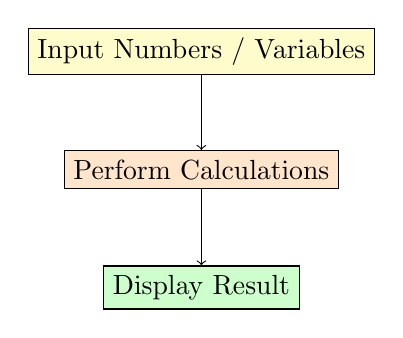
\begin{tikzpicture}[node distance=1.5cm]
\node (input) [draw, rectangle, fill=yellow!20] {Input Numbers / Variables};
\node (process) [draw, rectangle, fill=orange!20, below of=input] {Perform Calculations};
\node (output) [draw, rectangle, fill=green!20, below of=process] {Display Result};
\draw[->] (input) -- (process);
\draw[->] (process) -- (output);
\end{tikzpicture}
\end{center}

\section{Mini-Project: Simple Calculator Program}

Create a program that takes two numbers from the user and performs addition, subtraction, multiplication, division, and modulus:

\begin{verbatim}
# Simple Calculator
num1 = int(input("Enter first number: "))
num2 = int(input("Enter second number: "))

print("Addition:", num1 + num2)
print("Subtraction:", num1 - num2)
print("Multiplication:", num1 * num2)
print("Division:", num1 / num2)
print("Remainder:", num1 % num2)
\end{verbatim}

\section{Using Variables in Expressions}

Variables can be combined in expressions:

\begin{verbatim}
a = 10
b = 5
c = a + b * 2
print("Result:", c)
\end{verbatim}

Python follows \textbf{operator precedence} (multiplication/division before addition/subtraction).

\section{Key Concepts}

\begin{itemize}
    \item Expressions combine variables, values, and operators to calculate results.
    \item Python supports +, -, *, /, //, \%, ** operators.
    \item Variables can store inputs and results of calculations.
    \item Operator precedence affects the order of calculation.
\end{itemize}

\section{End-of-Chapter Exercises}

\begin{exercise}{Very Short Questions}
\begin{enumerate}
    \item Name three arithmetic operators in Python.
    \item What is the difference between / and //?
    \item What does the modulus operator (\%) do?
\end{enumerate}
\end{exercise}

\begin{exercise}{Short Answer Questions}
\begin{enumerate}
    \item Write a Python program to calculate the total of three exam marks.
    \item Explain operator precedence with an example.
    \item How do you store the result of a calculation in a variable?
\end{enumerate}
\end{exercise}

\begin{exercise}{Activity-Based Questions}
\begin{enumerate}
    \item Create a program to calculate your weekly pocket money remaining after spending on different items.
    \item Make a calculator program for two numbers performing all arithmetic operations.
    \item Modify the calculator to also calculate the average of the two numbers.
\end{enumerate}
\end{exercise}

\section{Teacher Notes}

\marginnote{
\textbf{Learning Objectives:} 
\begin{itemize}
    \item Students perform arithmetic operations in Python.
    \item Students understand expressions and operator precedence.
    \item Students combine input, variables, and calculations.
\end{itemize}

\textbf{Teaching Tips:} 
\begin{itemize}
    \item Demonstrate live calculations in Python.
    \item Encourage students to try different numbers to see how output changes.
\end{itemize}

\textbf{Assessment:} 
\begin{itemize}
    \item Check correctness of student calculator programs.
    \item Observe understanding of variable storage and operator precedence.
\end{itemize}
}